\chapter{\textsc{PF Eval}: Evaluating PF Tasks}
\label{chap:eval-framework}

\section{From Expert Task Review to Requirement Checks}
\label{sec:eval-overview}

In Chapter~\ref{chap:oneshot}, the rubric judge gave one-shot GPT-5 mini tasks an average score of $14.56$ out of $15$, even though many of these tasks could be solved with familiar methods, named the method students should use, or contained mathematical contradictions. An expert teacher would notice these problems when reviewing the tasks by hand, but such a review does not scale to the hundreds of tasks that an LLM can generate (Section~\ref{sec:intro-limitations}). We therefore need an automatic evaluation that tests whether a generated task works as a PF task, rather than how convincing its text reads.

To decide what this evaluation should test, we follow how a human designer checks a PF task (Section~\ref{sec:structpf-overview}). Instead of judging the task text as a whole, we turn the three PF requirements from Section~\ref{sec:intro-motivation} into separate questions, each with its own outcome, as decomposed checklists such as CheckEval~\cite{lee2025checkeval} and TICK~\cite{cook2024tick} do to make LLM judges more reliable. Figure~\ref{fig:eval-overview} summarizes these four designer questions and the automated checks that answer them.

\begin{figure}[!htb]
    \centering
    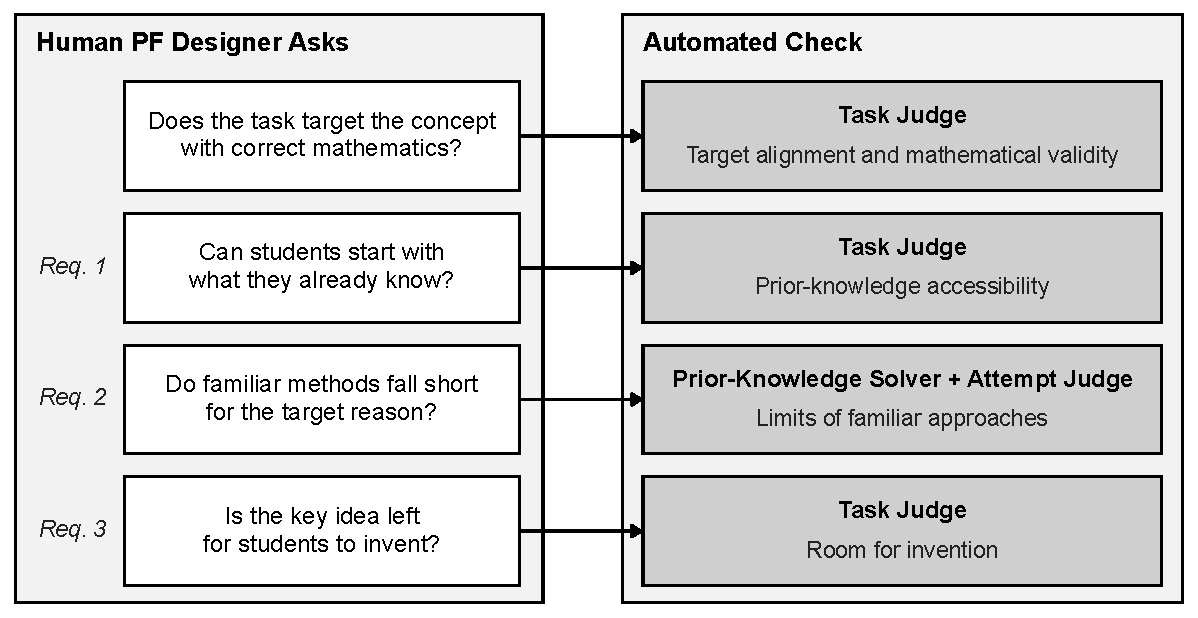
\includegraphics[width=0.92\textwidth]{figures/fig5_2_eval_overview.pdf}
    \caption[Mapping human PF designer questions to our five automated checks]{Mapping the four questions a human PF designer asks about a task to the five automated checks in \textsc{PF Eval}.}
    \label{fig:eval-overview}
\end{figure}

Three of the four questions in Figure~\ref{fig:eval-overview} can be checked directly from the task text and its numbers, whereas Requirement~2 cannot, because a judge that only reads the task never tries the familiar methods on the given values. Simulated students address this by letting an LLM attempt each item while playing a student with a given knowledge profile~\cite{lu2024,scarlatos2025smart}, but capable models in mathematics frequently leak knowledge beyond the assigned profile or abandon their errors (Section~\ref{subsec:bg-eval-simstudents}). More fundamentally, Requirement~2 asks about the task rather than about the students. As illustrated in Figure~\ref{fig:eval-simstudent-vs-solver}a, even when a simulated student stays within its profile, a solved or failed attempt remains ambiguous between student invention, leaked knowledge, and deliberate role-play mistakes. Our prior-knowledge solver (Figure~\ref{fig:eval-simstudent-vs-solver}b) instead tests the task directly by doing its best with only the listed prior procedures and no deliberate errors, while a separate attempt judge that knows the target concept sets aside any attempt that uses an unlisted concept. Section~\ref{sec:eval-five-measures} defines the five task-design measures behind Figure~\ref{fig:eval-overview}, Section~\ref{sec:eval-three-roles} describes the prior-knowledge solver and the two judges, and Section~\ref{sec:eval-validation} validates \textsc{PF Eval} as a whole.

\begin{figure}[!htb]
    \centering
    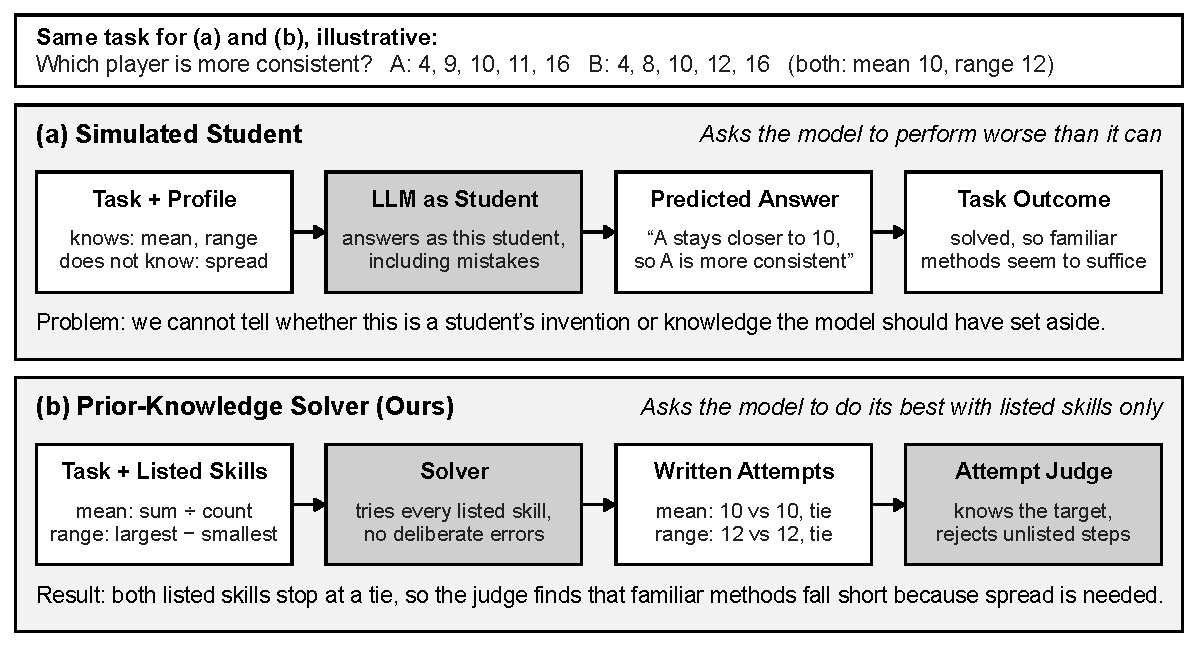
\includegraphics[width=0.92\textwidth]{figures/fig5_1_simstudent_vs_solver.pdf}
    \caption[Simulated student persona versus our prior-knowledge solver on consistency]{Comparison of (a)~a role-play simulated student and (b)~our target-blind prior-knowledge solver on the illustrative consistency task.}
    \label{fig:eval-simstudent-vs-solver}
\end{figure}

\section{Five Task-Design Measures}
\label{sec:eval-five-measures}

To evaluate a generated task against the questions in Figure~\ref{fig:eval-overview}, we need measures that show which requirement holds and which fails. We have chosen to evaluate each question as a separate measure with its own outcome (\emph{Yes}, \emph{No}, or \emph{Unclear}) rather than summing points into a single score, because a high total can hide a failure on one requirement, as we saw with the $14.56 / 15$ rubric average in Chapter~\ref{chap:oneshot}. Table~\ref{tab:eval-five-measures} defines the five measures. The first two measures verify that the problem addresses the target concept with consistent mathematics, since a task that teaches the wrong concept or contradicts itself cannot be productive, while the remaining three test Requirements~1 to~3 directly.

\begin{table}[!htb]
\centering
\caption[Definitions of the five task-design measures in \textsc{PF Eval}]{Definitions of the five task-design measures testing target alignment, mathematical validity, and PF Requirements~1 to~3.}
\label{tab:eval-five-measures}
\vspace{0.5em}
\footnotesize
\setlength{\tabcolsep}{8pt}
\renewcommand{\arraystretch}{1.2}
\begin{tabularx}{\linewidth}{@{} >{\raggedright\arraybackslash}p{0.28\linewidth} >{\raggedright\arraybackslash}X @{}}
\toprule
\textbf{Measure} & \textbf{Definition} \\
\midrule
Target alignment & Solving the task's central problem requires the target concept, even when the task never names it \\
\addlinespace[5pt]
Mathematical validity & The givens are consistent with each other, and the task has at least one solution \\
\cmidrule(l{0pt}r{0pt}){1-2}
Prior-knowledge accessibility (Req.~1) & A student can make a meaningful start on the task using the listed prior skills and basic arithmetic \\
\addlinespace[5pt]
Limits of familiar approaches (Req.~2) & A familiar method, carried out correctly, falls short for the reason that the target concept resolves \\
\addlinespace[5pt]
Room for invention (Req.~3) & The task leaves its central construction, such as a measure, model or fair rule, for students to build \\
\bottomrule
\end{tabularx}
\end{table}

Evaluating a PF task on these measures differs from reviewing a standard textbook exercise, where the prompt usually names the method to apply and admits a single prescribed procedure. In a PF task, withholding the target concept and leaving the comparison rule open, such as letting students decide how to measure consistency in Figure~\ref{fig:eval-simstudent-vs-solver}, are deliberate design features rather than omissions or ambiguities. This is why the definition of target alignment in Table~\ref{tab:eval-five-measures} does not require the task to name the target concept, and why we treat an intended open choice of method as mathematically valid rather than underspecified. In order to distinguish prompts that give away the entire method from prompts that only narrow the student's search, we also include a middle outcome (\emph{Partly}) for room for invention when a task states a hint or target criterion while still leaving a secondary decision open.

We also need to ensure that a failed prerequisite check or an incomplete problem statement is not confused with a failed PF mechanism. We have therefore chosen to evaluate the five measures in a fixed order and to keep \emph{Unclear} separate from \emph{No}. In particular, we check mathematical validity only when a task is aligned with the target concept, and we test the limits of familiar approaches only when the task is accessible with prior knowledge, because a familiar method cannot meaningfully fall short on a problem that students cannot even start. When an earlier check fails, the dependent measure is recorded as \emph{not assessed} rather than \emph{No}. Similarly, when essential context such as a referenced diagram is missing, we return \emph{Unclear} so that uncertainty in the judge is not counted as a confirmed flaw in the task.

\section{Prior-Knowledge Solver and Evaluation Judges}
\label{sec:eval-three-roles}

The five measures are answered by three LLM roles, which we separate by what each role must not see. The task judge does not see the solver's attempts, so that its outcomes rest on the task text rather than on how one solver happened to perform. The solver does not see the target concept, because a model that knows the goal would steer towards it, and its attempts would no longer show what the familiar methods achieve on their own. Only the attempt judge sees everything, because it must decide whether an attempt falls short for the reason that the target concept resolves.

An illustration of the entire process is shown in Figure~\ref{fig:eval-three-roles}. Every task undergoes this process, which has two parts. First, the task judge reads the task and returns the outcomes for four of the five measures. Second, if the task is accessible, the solver attempts it with the listed skills, and the attempt judge labels each attempt, from which the outcome for the limits of familiar approaches follows.

\begin{figure}[!htb]
    \centering
    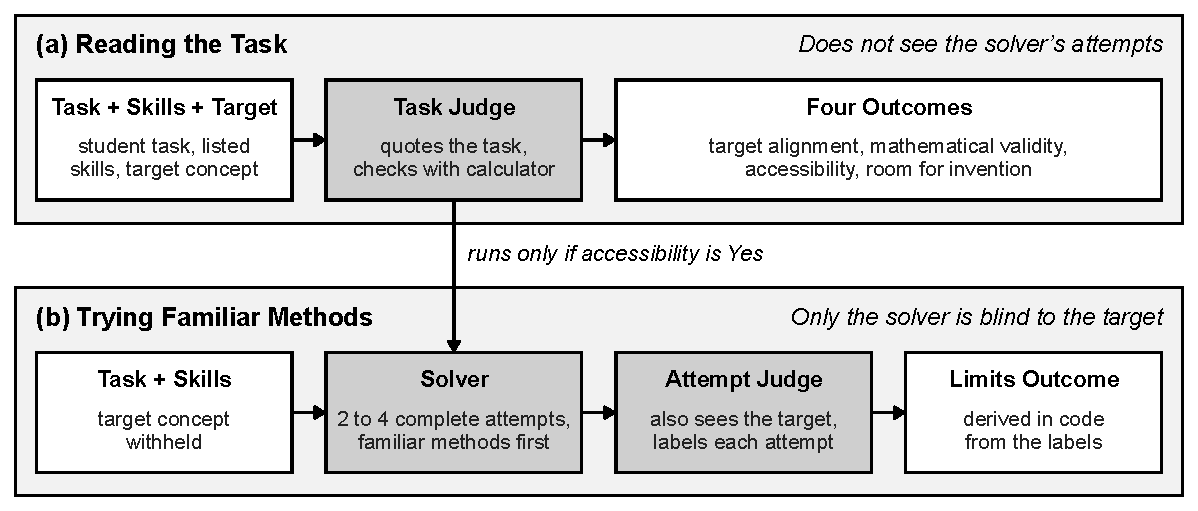
\includegraphics[width=0.92\textwidth]{figures/fig5_3_three_roles.pdf}
    \caption[Information separation across the task judge, solver, and attempt judge]{Information separation across the three evaluation roles: the task judge~(top) and the target-blind solver plus attempt judge~(bottom).}
    \label{fig:eval-three-roles}
\end{figure}

\subsection{Task Judge}
\label{subsec:eval-task-judge}

For target alignment, accessibility, and room for invention, we require the task judge to quote the exact phrases from the student task that support its outcome, and our evaluation code verifies that every quoted phrase appears in the task text. Grounding each outcome in verbatim quotes prevents the judge from inferring support or hints that are not written in the prompt. For mathematical validity, the judge translates numerical claims in the problem into checks for the \texttt{SymPy} calculator from Section~\ref{subsec:d2b-numbers}, so that conditions such as two equal means are computed exactly rather than estimated by the language model.

\subsection{Prior-Knowledge Solver}
\label{subsec:eval-solver}

On tasks that pass the accessibility check, the prior-knowledge solver generates between two and four complete attempts that each answer every part of the task. We divide these attempts into two ordered tiers because a single familiar method and a combined strategy test different aspects of the task design.
\begin{enumerate}[leftmargin=0.6cm,itemsep=0.4em,topsep=0.4em]
    \item \textbf{Familiar Methods}\\[0.2em]
    The first attempts apply a single listed method on its own, such as comparing only the means or only the ranges in the consistency task, and record where that method falls short.
    \item \textbf{Constructed Approaches}\\[0.2em]
    The remaining attempts combine several listed skills or apply general problem-solving heuristics, such as guessing and testing candidate values or organizing the givens in a table~\cite{polya1945}, to see whether a working solution can be constructed from prior knowledge.
\end{enumerate}

When the listed prior skills already include a procedure that solves the task directly, the solver applies that taught procedure across all parts of the problem rather than inventing an artificially weakened baseline, ensuring that a routine textbook exercise is not mistaken for a PF task. Each attempt states the mathematical principle it relies on and any assumptions it makes, and the solver may call the calculator one arithmetic step at a time, just as a student would use a pocket calculator.

\subsection{Attempt Judge}
\label{subsec:eval-attempt-judge}

Because the solver is blind to the target concept, a separate attempt judge inspects each attempt against the target concept and assigns one of the five labels in Table~\ref{tab:eval-attempt-labels}.

\begin{table}[!htb]
\centering
\caption[Attempt-judge labels and their effect on the familiar-limits outcome]{Attempt-judge labels assigned to each solver attempt and their effect on the outcome for the limits of familiar approaches.}
\label{tab:eval-attempt-labels}
\vspace{0.5em}
\footnotesize
\setlength{\tabcolsep}{8pt}
\renewcommand{\arraystretch}{1.2}
\begin{tabularx}{\linewidth}{@{} >{\raggedright\arraybackslash}p{0.15\linewidth} >{\raggedright\arraybackslash}X >{\raggedright\arraybackslash}X >{\raggedright\arraybackslash}p{0.18\linewidth} @{}}
\toprule
\textbf{Label} & \textbf{When Assigned} & \textbf{Example Attempt} & \textbf{Effect on Outcome} \\
\midrule
Target limit & A correct familiar method falls short for the reason that the target concept resolves & Compares the means, 10 and 10, and finds a tie that only a measure of spread can break & Yes, even if other attempts solve the task \\
\addlinespace[5pt]
Meets demands & Correct reasoning with the listed skills answers the task & Adds each score's distance from 10, giving 14 for A and 16 for B, so A is more consistent & No, if no attempt is a target limit \\
\addlinespace[5pt]
Unresolved & The attempt stops after a setup step, or its start cannot be checked & Sorts each player's scores and stops before comparing the players & Unclear, if no attempt is a target limit \\
\cmidrule(l{0pt}r{0pt}){1-4}
Unrelated shortfall & The attempt falls short for a reason that the target concept does not address & Stops because the task misstates A's mean as 11 & None, since the flaw lies outside the target \\
\addlinespace[5pt]
Unsupported & The attempt uses an unlisted concept, misreads the numbers, or makes no mathematical move & Applies the standard deviation formula, which is not a listed skill & None, since the attempt leaves the listed skills \\
\bottomrule
\end{tabularx}
\end{table}

Code then derives the outcome for the limits of familiar approaches from the rules in the last column of Table~\ref{tab:eval-attempt-labels}: a single \emph{Target limit} is enough for \emph{Yes} even if a later constructed attempt also \emph{Meets demands}, whereas a routine task where familiar methods reach \emph{Meets demands} directly without any \emph{Target limit} receives \emph{No}.

Finally, two practical boundaries of this three-role design should be noted before we validate \textsc{PF Eval} in Section~\ref{sec:eval-validation}. First, because the solver explores at most four approaches per run, a missing \emph{Target limit} can occasionally reflect an approach the solver did not try rather than a flaw in the task. Second, the attempt judge can only flag an untaught concept when that concept is visible in the solver's written steps. We therefore interpret the resulting outcomes as evidence about the task's mathematical structure under the listed skills, rather than as a prediction of classroom behavior.

\section{Validating \textsc{PF Eval}}
\label{sec:eval-validation}

Since every outcome in \textsc{PF Eval} comes from LLM roles, we need to show that these outcomes can be trusted before we use them to compare generators in Chapter~\ref{chap:results}. A low pass rate could mean that the generated tasks are weak, but it could equally mean that \textsc{PF Eval} is too strict, and a high pass rate could likewise come from a lenient \textsc{PF Eval}. We therefore validate \textsc{PF Eval} in two steps matching the two subsections below: first, we test whether the prior-knowledge solver finds the expected student approaches on its own (Section~\ref{subsec:val-solver}), and second, we test whether \textsc{PF Eval} as a whole accepts published PF tasks and rejects flawed tasks for the right reason (Section~\ref{subsec:val-known-tasks}).

\subsection{Testing the Solver on Expected Approaches}
\label{subsec:val-solver}

\textsc{PF Eval} can only return \emph{Yes} on the limits of familiar approaches when the solver actually tries a familiar method that falls short, and it can only return \emph{No} on a routine task when the solver finds the routine solution (the first boundary in Section~\ref{sec:eval-three-roles}). To test the solver separately from the rest of \textsc{PF Eval}, we built a benchmark of 76 tasks and recorded 256 expected approaches before running the solver, covering student solutions from the PF literature for published PF tasks, standard solutions for routine and control tasks, and the planned Step~2a approaches (Section~\ref{subsec:d2a-brief}) for pipeline-generated tasks. We run the solver exactly as in \textsc{PF Eval}, pooling attempts from GPT-5.6-luna and GPT-4.1 without tuning on this benchmark, and use a matching judge to check whether each expected approach is carried out.

\begin{figure}[!htb]
    \centering
    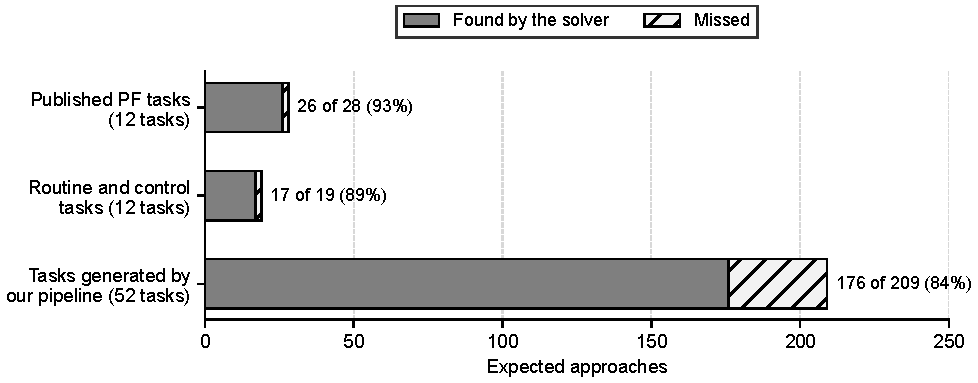
\includegraphics[width=0.9\textwidth]{figures/fig5_4_solver_recall.pdf}
    \caption[Recovery of expected student approaches by the prior-knowledge solver]{Proportion of 256 expected approaches recovered by the pooled prior-knowledge solver across 76 benchmark tasks ($85.5\%$ overall).}
    \label{fig:val-solver-recall}
\end{figure}

As shown in Figure~\ref{fig:val-solver-recall}, the solver recovers $85.5\%$ of the expected approaches overall, with nearly all misses occurring on the pipeline-generated tasks whose planned approaches were written by the generator rather than observed in students. More importantly for task evaluation, on every PF task in the benchmark (including all published tasks), the solver tries at least one familiar method that falls short as required for a \emph{Yes} on the limits of familiar approaches, and on every routine task it finds the direct solution without inventing artificial failures. Manual inspection of a 12-task sample also confirmed all matching decisions.

\subsection{Validating \textsc{PF Eval} on Reference Tasks}
\label{subsec:val-known-tasks}
\label{subsec:val-good-pass}
\label{subsec:val-flawed-fail}

To test \textsc{PF Eval} as a whole, we collected the 29 reference tasks summarized in Table~\ref{tab:eval-known-tasks}, which pair published PF tasks~\cite{puech2025} against routine textbook versions~\cite{kapur2012}, flawed one-shot tasks from Chapter~\ref{chap:oneshot}, single-flaw control tasks, and two \textsc{StructPF} tasks, with expected outcomes fixed from the source papers and task text. Figure~\ref{fig:val-reference-outcomes} reports the resulting non-passing counts by group, where an empty cell means every assessed task in that group received \emph{Yes}.

\begin{table}[!htb]
\centering
\caption[Reference task groups used to validate \textsc{PF Eval}]{Reference task groups ($N = 29$) with known strengths and flaws used to validate \textsc{PF Eval}.}
\label{tab:eval-known-tasks}
\vspace{0.5em}
\footnotesize
\setlength{\tabcolsep}{8pt}
\renewcommand{\arraystretch}{1.2}
\begin{tabularx}{\linewidth}{@{} >{\raggedright\arraybackslash}p{0.17\linewidth} >{\centering\arraybackslash}p{0.06\linewidth} >{\raggedright\arraybackslash}X >{\raggedright\arraybackslash}p{0.27\linewidth} @{}}
\toprule
\textbf{Group} & \textbf{Tasks} & \textbf{Example} & \textbf{Expected Outcome} \\
\midrule
Published PF tasks & 12 & Design a measure of consistency for three football players~\cite{puech2025} & Yes on all five measures, with Unclear validity for one task \\
\addlinespace[5pt]
Routine versions & 3 & Find a ship's average speed over a journey with two parts~\cite{kapur2012} & No on limits and room for invention \\
\addlinespace[5pt]
One-shot tasks & 5 & The garden task in Figure~\ref{fig:oneshot-math-error-example} & No on limits, and a failing outcome for each further flaw \\
\addlinespace[5pt]
Control tasks & 7 & Show a rectangle of 3~cm by 2~cm with an area of 5~cm$^2$ & No or Unclear on the measure that each task breaks \\
\addlinespace[5pt]
\textsc{StructPF} tasks & 2 & Invent a consistent rule for multiplying negative numbers & Yes on all five measures for one task, No on limits for the other \\
\bottomrule
\end{tabularx}
\end{table}

\begin{figure}[!htb]
    \centering
    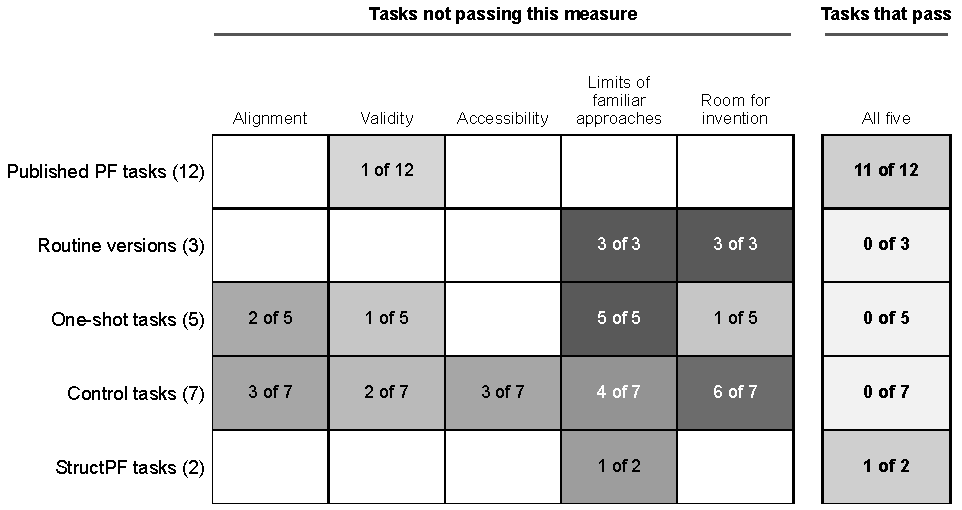
\includegraphics[width=0.9\textwidth]{figures/fig5_5_reference_outcomes.pdf}
    \caption[\textsc{PF Eval} outcomes across the 29 reference tasks by task group]{Non-passing measure counts and overall pass counts across the five reference task groups ($N = 29$ tasks; empty cells indicate all tasks pass).}
    \label{fig:val-reference-outcomes}
\end{figure}

The outcomes in Figure~\ref{fig:val-reference-outcomes} confirm both requirements for \textsc{PF Eval} to be reliable:

\begin{enumerate}[leftmargin=0.6cm,label=\textbf{\arabic*.},itemsep=0.6em,topsep=0.4em]
    \item \textbf{Accepting Published PF Tasks}\\[0.2em]
    As shown in the top row of Figure~\ref{fig:val-reference-outcomes}, all published PF tasks pass every measure except for one \emph{Unclear} validity outcome on the hummingbird migration task. Because that task gives each bird's wing beats per minute only as an interval (such as 70 to 80), the resulting daily distances overlap and the winner depends on which values a student picks, so returning \emph{Unclear} rather than \emph{No} matches the task's actual mathematical structure.

    \item \textbf{Rejecting Flawed Tasks for the Right Reason}\\[0.2em]
    Across the lower rows of Figure~\ref{fig:val-reference-outcomes}, none of the flawed tasks passes all five measures, and each group fails on the specific measure its flaw targets. For example, when the published consistency task is modified only by spelling out the variance rule step by step, the task judge quotes \emph{``use exactly this rule''} to return \emph{No} on room for invention and the solver applies that rule directly to return \emph{No} on the limits of familiar approaches, while the $15 / 15$-rated one-shot Garden task~28 (Figure~\ref{fig:oneshot-math-error-example}) is rejected on both familiar limits and mathematical validity.
\end{enumerate}

Across all 29 reference tasks, \textsc{PF Eval} matches every expected outcome, accepting the published PF tasks while rejecting the routine, one-shot, and control tasks on the exact measures they violate. One limitation of this check is that the 29 tasks and their expected outcomes were compiled from the source papers and used while refining the judge prompts, rather than being rated by an independent group of teachers on an unseen test set. Having verified that the solver finds expected familiar approaches (Section~\ref{subsec:val-solver}) and that the three roles separate working PF tasks from flawed ones, we use \textsc{PF Eval} in Chapter~\ref{chap:results} to compare \textsc{StructPF} against one-shot generation.
